\documentclass{minimal}
\usepackage[spanish]{babel}
\usepackage{graphicx}
\usepackage[utf8]{inputenc}
\usepackage{fancyhdr}
\usepackage{lastpage}

\pagestyle{fancy}
\fancyhf{}
\rfoot{Page \thepage\hspace{1pt} de~\pageref{LastPage}}

\title{Practica 6}
\author{Guillermo Lopez Garcia}
\begin{document}
\maketitle

\textbf{Ejercicio 1.} \\
- Respecto al problema de los numeros primos, la tipología del problema es claramente de calculo numerico. La solución por la que
se ha optado es una solución de multi-hebra, calculando en cada hebra una serie de numeros primos en un rango determinado. Y para 
la ecuación $N_{t} = \frac{N_{nld}}{1-C_{b}}$, obtenemos que, para en mi caso, con 8 hilos de ejecución con un $C_{b}=-1$, conseguiriamos
4 hilos de ejecución calculando una cuarta parte de los números primos del rango total en cada hilo.\\

- Respecto al problema de las paginas web, la tipologia del problema es claramente de retardos en operaciones de entrada-salida. La
solución por la que se ha optado es una solución multi-hebra, donde en cada hebra se obtienen los datos de cada pagina web y lo introduce
en un fichero. Para la ecuación $N_{t} = \frac{N_{nld}}{1-C_{b}}$, obtenemos que si queremos un hilo para cada pagina web, El $C_{b}$ debe ser
igual a 0.2. Esta es la mejor aproximación al coeficiente, ya que, con menos hilos de ejecución tardamos mas y con mas hilos de ejecución
provocamos mas cambios de contexto en la CPU provocando a su vez mayor tiempo para la finalización del programa.\\
\\


A continuación, expongo la grafica generada con gnuplot para mostrar comparación entre 
tiempo y Speed Up.
\\
\begin{figure}
  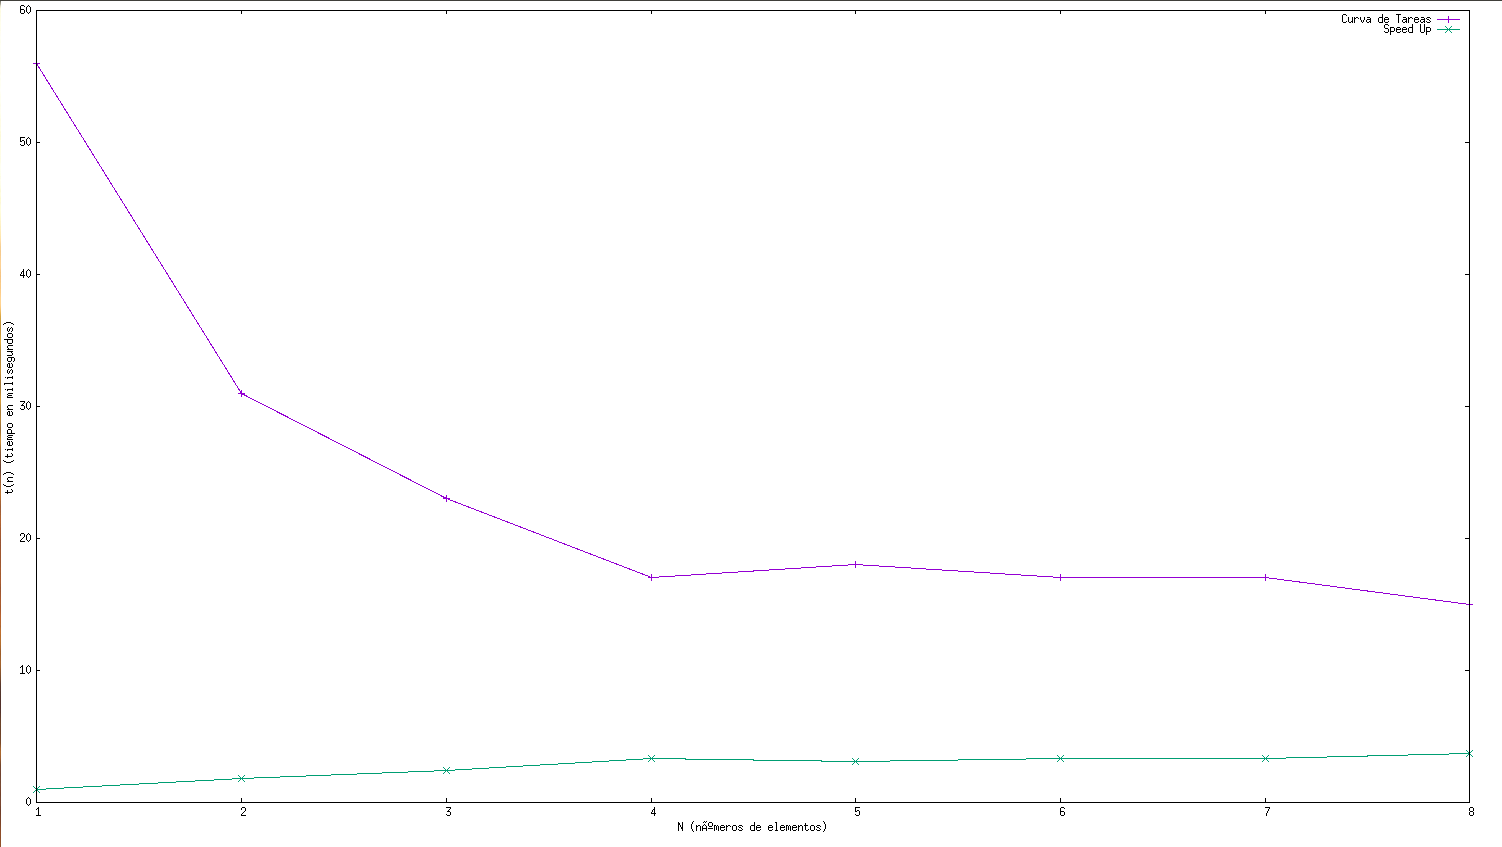
\includegraphics[width=\linewidth]{img.png}
  \caption{Comparativa de Speed Up y Tiempo.}
\label{fig:comp}
\end{figure}
\\
\\
Por último solo he podido probar el funcionamiento en un sistema Linux. No tuve acceso al sistema privativo y de licencia pagada Windows.

\end{document}
